\chapter{Evaluation}
This chapter deals with evaluating the results from the program when scoring article comparisons.

After having done tests to verify that the implementation of the algorithms worked correctly, it is now time to analyse the output.

\section{Scores}

The Cosine algorithm returns a score that is in fact an angle, where as the LCS algorithm returns a score that is based on the length of a string. As such these are hardly comparable in a one to one basis. If we modify the score of the LCS to not say something about the length of the substring(s), but tell us in percent how long the string is compared to the article is, it will produce a result that relates to the amount of text the two articles being compared have in common. This being said we still need to consider that the percentage value is relative to the length of the length of the article. We do therefore need to do a percentage calculation for both article's length. For better comparison of the Cosine and LCS score in the Excel graphs, the LCS percentage score is divided by 100 (even though comparing the scores is not really a decent indicator, it helps giving a better overview of the graphs).

So, a Cosine score of 1.0 means that the two article vectors are identical, same length and no angle between them. A LCS score of 1.0 means that the longest common substring's length is 100\% of the article's length. So each score will have to be evaluated on their own premisses, as a Cosine score of 0.5 is not 50\% identical. The Cosine score tells us something about how many special words that two articles have in common, where are the LCS tells us about the amount of text (substrings) that is shared between the two articles.

\section{Limiting the Number of Comparisons by Cosine Score}

As discussed in the last chapter (see section ~\ref{AllFractiles}) there is many comparisons in the lowest fractile of the article comparisons. Although dismissing them right of the bat can be seen as hasty, the chance of comparisons scoring below 0.3 having much in common would be unlikely. This is because comparisons that score very low in the Cosine algorithm either have very little in common in terms of special words (as common words will have very little impact on the vector) or the article is very short and again, with few special words (we will see an example of this later on). However, an article with no special words that is very short, is very rare and few in between. We will however see examples of such articles later on.

For the sake of proving anything in this thesis how ever, and as the chance of getting useful results from comparisons with low Cosine scores are slim and the number of comparisons having to be humanly checked are massive in numbers should we check all comparisons, I will for the rest of this thesis, disregard all comparisons with a cosine score lower than 0.3.

\section{What the Scores Tell}
First off we need to realize what the different scores is telling us on their own. The cosine score will give an indication of how similar two articles are in regards to the words being used, but will not tell us anything in regards to what the article is actually saying in regards to the structure of sentences (see section ~\ref{CosineProblem}). By it's own, Cosine will tell us more about if the comparisons have the same topic that actually the same sentences. 

The modified LCS is an indication of how big a percentage of text in relation to article length that an article have in common with another article. The LCS score will therefore tell us a lot about how much actual text a comparison shares. 

\subsection{Definition of "High Scoring"}
A lot of the results in the result sets, are subject to a lot of "gut feelings". There will be mentions of "high" score values. This is of course a relative term, because when can we truly define a score as high? For the Cosine part a high score would be 0.9 and higher. Below that we can start to see gray areas in which the score is not definite any more. When speaking of high scores in the LCS values things start to become even more fuzzy. A LCS score of 0.3 might be telling a lot in articles that is very long, but in very short articles, that score might just mean a single substring consisting of few words. The term high should in this relation be considered on a basis of the score value and the length of the article. This issue will be discussed later.

\section{Score Analysis}

In figure ~\ref{SubstringsEx} we see a part of the LCS result of two articles being compared with each other. A long each axis we have an article (topmost row and leftmost column - not visible on image). The purple squares shows where a word match have been found, and a diagonal row of coloured squares indicate several words in concession have been found. If squares are coloured in purple, it means that the substring found is too short, if the squares are in brown the substring is equal to or greater than the threshold set for accepting substrings.

In the figure we see that the two articles start off with having a lot in common, then around two thirds into figure there is a huge gap along the x-axis, but it is largely unbroken along the y axis. So if judging the result by looking at this image we can establish two things.

\begin{itemize}
\item The two articles have a lot of text in common, but the article along the x-axis is substantially longer than the article along the y-axis.
\item The article along the y-axis is an excerpt of the article along the x-axis.
\end{itemize}

So when looking at this plot, we can tell if an article comparison is a duplicate, a excerpt or if there is no real match between two articles. To validate this fully it is needed to read the article text, to make sure the combination of substrings is not just a collection of random words, that are aligned in the same way without any relation.

In the following when looking at LCS comparison of articles, they are plotted like this in Excel. 

\section{Analysis of Comparisons}
In the following is described the evaluation of the scores produced by matching the four sources (JP being matched with POL and JV being matched with FL). In this section there will be a lot of references to Excel files. These are included in the electronic version of this thesis. In the two files containing the comparisons for all articles in the source folders (File: JPPOL.xlsx and JV-Lemvig.xlsx), some of the comparisons are marked with \textit{Match}, \textit{PartialMatch}, \textit{SameContent} and \textit{LowScoreMatch}. These comparisons have been plotted in Excel as well, and they are included in their respective source folders labelled with that match name and the name of the files is the combination of the ids in the comparisons.

\subsection{JP and POL Comparison}
First off, the sources POL and JP was compared in the program. The results of this was then plotted in Excel (File: JPPOL.xlsx). The data columns are:

\begin{itemize}
\item \textbf{Left Id / Right Id:} The article Ids of the comparison. These are used to find the articles, when checking their content manually.
\item \textbf{Cosine Score:} The Cosine score for the comparison.
\item \textbf{LCS Score:} The unmodified LCS score. This is included for comparison with the modified LCS score. It is a percentage score off the longest of the two articles in the comparison.
\item \textbf{Combined Score Max:} The score from the modified LCS. This is a percentage score off the longest of the two articles in the comparison.
\item \textbf{Combined Score Min:} The score from the modified LCS. This is a percentage score off the shortest of the two articles in the comparison.
\item \textbf{Long Length:} The length of the longest article in characters.
\item \textbf{Short Length:} The length of the shortest article in characters.
\item \textbf{Match Group:} The match group the comparison have been placed into by the program (this will be explained later).
\item \textbf{Adjusted Score:} The score modification after applying score weighing (this will also be explained later).
\end{itemize}

Originally only the LCS score based off the longest article was included and used for evaluating the results. It did become clear after the first few tests, that this would not suffice. If we looked at two articles, one being substantially longer than the other, but the shortest being a 100\% excerpt of the longest, we could end up in a case where the article comparison would score very low because the LCS (and the Cosine for that matter) would be very low. We could then end up discarding this comparison as a "no match" because the scores was too low. How ever if we looked at the LCS score based off the length of the shortest article, we would get a completely different image. Then we could actually detect that the shortest article was in fact a excerpt, by seeing that it's LCS score would be 100\%. We will therefore have to look into the length of the articles as well, in order to fully say something about how much of a match a comparison is (this will be brought up again later).

Finally there are three graphs. The first is \textit{'Sample Distribution with Stopwords'}. This shows in a column diagram the comparisons different scores. As mentioned earlier we cannot compare the Cosine score with the LCS score on a one to one basis. However this does indicate something about general relations.

\begin{figure}
	\centering
	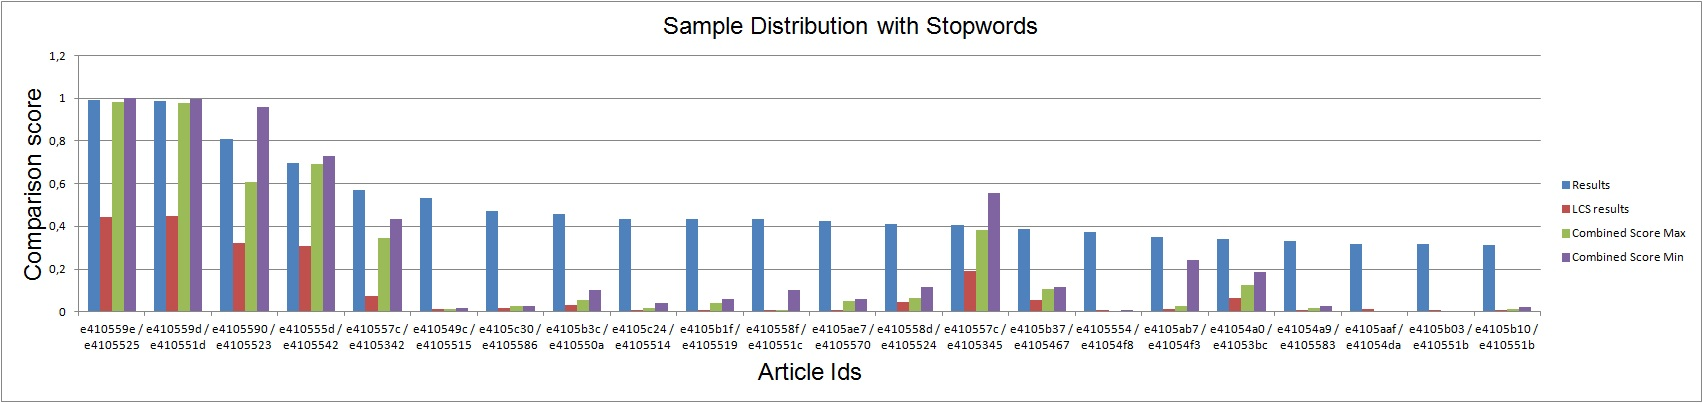
\includegraphics[scale=0.25]{figures/JPPOLScoreGraph}
	\caption{Comparison scores for the JP and POL sources (see appendix D for bigger image or File: JPPOL.xlsx).}
	\label{JPPOLScoreGraph}
\end{figure}

Figure ~\ref{JPPOLScoreGraph} shows the effect of having the modified LCS to collect all substrings longer than a given threshold. It also shows the necessity of having to evaluate the LCS score with both the length of the longest and the shortest article length as there can be quite a big difference in the scores.

Below that graph is two graphs side by side. The first shows the Cosine score plotted with the modified LCS score based off the longest article. The second graph shows the same, but this time the red dots is showing the Cosine and modified LCS score based off the shortest article.

The graphs in figure ~\ref{MaxScore} and ~\ref{MinScore} was created in order to get a better overview of how the scores was distributed. 

\begin{figure}
	\centering
	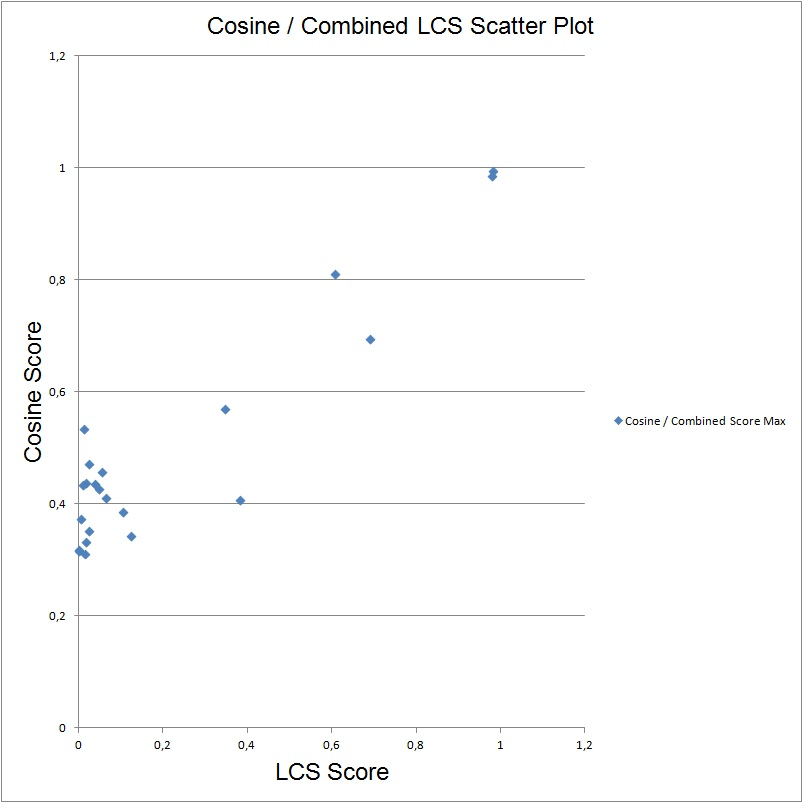
\includegraphics[scale=0.5]{figures/JPPOLCosineLCSMax}
	\caption{A plot showing the Cosine / LCS score (based of the longest article length in the comparison).}
	\label{MaxScore}
\end{figure}

\begin{figure}
	\centering
	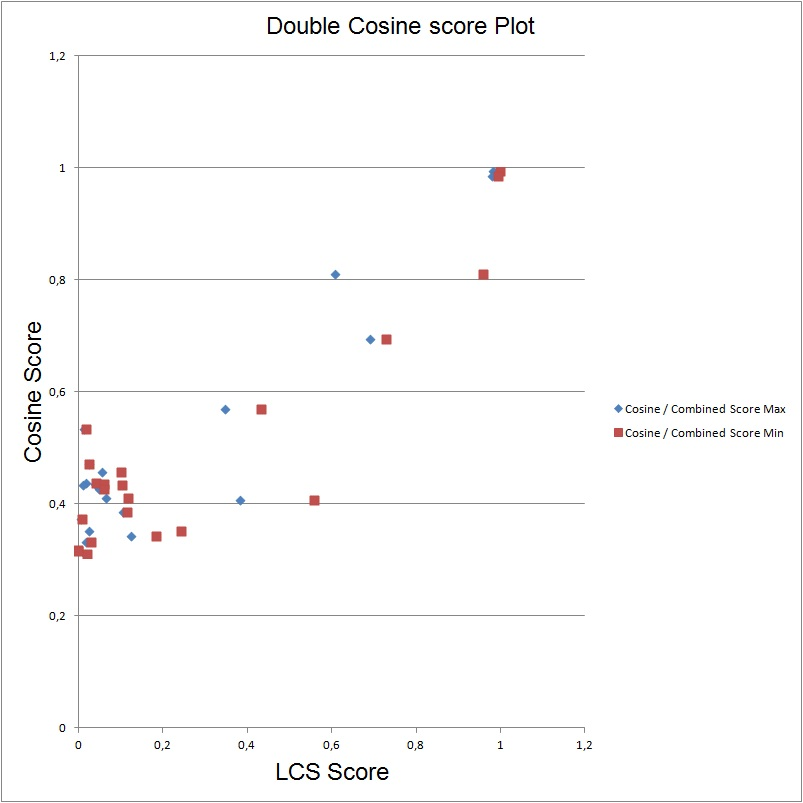
\includegraphics[scale=0.5]{figures/JPPOLCosineLCSMin}
	\caption{A plot showing the Cosine / LCS score (based off the longest article length - the blue dots) and the Cosine / LCS score (based off the shortest article length - the red squares).}
		\label{MinScore}
\end{figure}

When evaluating the figure ~\ref{JPPOLScoreGraph} we can start with looking at the first two collections of scores (comparisons \textit{e410559e / e4105525} and \textit{e410559d / e410551d}). Both comparisons have high scores in all columns. We note that the basic LCS scores around half as high as the scores for the two modified LCS scores. For the rest of this thesis I will disregard the scores produced by the basic LCS, as it holds no meaningful data when trying to find article duplicates. The length of the four articles in the comparisons is around the same length, meaning both of the LCS scores is more or less equally high.

The thesis about the algorithm scores can be now be verified. From the excel file we get the scores seen in table ~\ref{JPPOLHighScores} and table ~\ref{JPPOLSecondHighestScores}. The scores is sorted by Cosine score. 

\begin{table}
\begin{center}
	\begin{tabular}{l | r}
	Ids & e410559e / e4105525\\ \hline
	Cosine & 0.992916226\\ \hline
	Basic LCS & 0.441762865\\ \hline
	LCS (long article) & 0.981112301\\ \hline
	LCS (short article) & 0.998931646\\ \hline
	Long article length & 953\\ \hline
	Short article length & 936\\ \hline	
	\end{tabular}
\end{center}
\caption{Scores for the highest scoring article comparison when comparing JP and POL sources (File: JPPOL.xlsx). The two last LCS scores is the LCS score percentage based off the longest article, and the scored based off the shortest article.}
\label{JPPOLHighScores}
\end{table}

\begin{table}
\begin{center}
	\begin{tabular}{l | r}
	Ids & e410559d / e410551d\\ \hline
	Cosine & 0.985605299\\ \hline
	Basic LCS & 0.449531734\\ \hline
	LCS (long article) & 0.979188323\\ \hline
	LCS (short article) & 0.994714558\\ \hline
	Long article length & 961\\ \hline
	Short article length & 936\\ \hline	
	\end{tabular}
\end{center}
\caption{Scores for the second highest scoring article comparison when comparing JP and POL sources (File: JPPOL.xlsx).}
\label{JPPOLSecondHighestScores}
\end{table}

When looking at table ~\ref{JPPOLHighScores} all the algorithm scores are high, all near 1.0 (except from the basic LCS score which we disregard). The articles are of similar length and they have a length that indicates that they contain a lot of text. To begin with, we will evaluate the results by looking at the LCS plot.


\begin{figure}
	\centering
	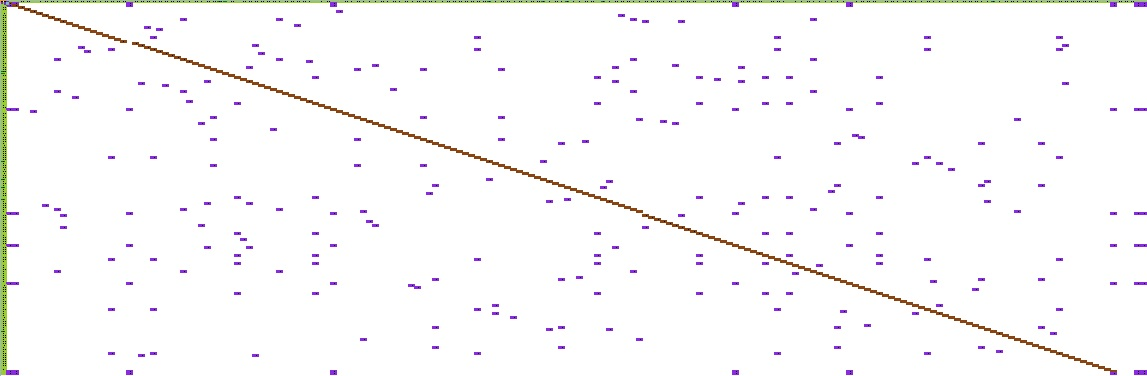
\includegraphics[scale=0.35]{figures/e410559e}
	\caption{Plot of the result of comparing article e410559e and article e4105525 using the LCS algorithm (File: e410559e-e4105525.xlsx). See appendix ~\ref{D2} for a bigger image.}
	\label{JPPOLHighestLCS}
\end{figure}

The plot ~\ref{D2} clearly shows a diagonal line going from top left towards bottom right. There are a few minor deviances along the way, which corresponds well with what the LCS score tells us, that the we are just a tiny bit away from having a 100\% perfect match. 

After the initial verification, comes the task of manually checking the content of the articles to make sure that they are in fact (almost) identical. The article text can be found in appendix ~\ref{JPPOLHighestMatch1} and appendix ~\ref{JPPOLHighstMatch2}. After reading the text it is clear that the texts are in fact identical, except from the very last sentence in the first article ~\ref{JPPOLHighestMatch1} which only contains an email, but then what about the two breaks in the middle of the comparisons? This is where the issue of text normalization becomes evident. The differences marked by the LCS is actually caused by the way the XML files containing the article text is read. In the figures ~\ref{XmlIssue1} and ~\ref{XmlIssue2} we can see that one article have a paragraph break in a sentence that the other article does not have. The way that text is being extracted by the Cosine algorithm (it is a part of the program that does the Cosine comparison that also extracts the text from the XML files, this is of course done before the comparison is made, and is a part of the system that was not implemented in this thesis), removes non alphabetic characters, in this case the punctuation. In the other article the paragraph also ends with a punctuation, but when that is removed, there is no word following the last word in the paragraph like in the other article. This means that one article will then have a white space that is not present in the other article. In order to fix this, text should be normalized in a way that makes sure that all paragraph breaks inserts a white space into the text if one is not present already. If that had been done, the LCS score would have been higher. This problem is present in a lot of the results, but is unlikely to cause a significant error source (but should be kept in mind). This problem is frequently occurring in article duplicates, as articles will be broken into paragraphs that might fit the layout of the paper, or due to other reasons.

\begin{figure}
	\centering
	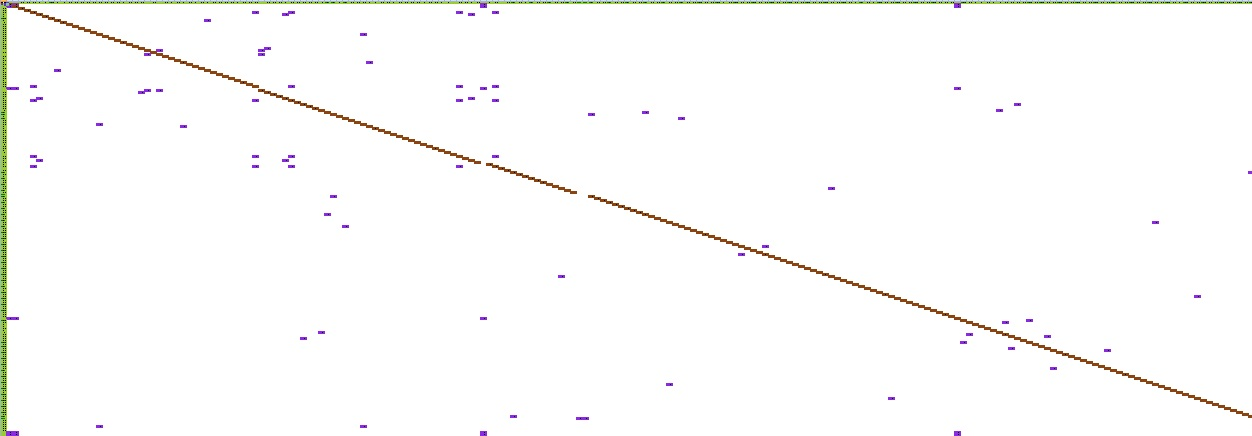
\includegraphics[scale=0.35]{figures/e410559d}
	\caption{Plot of the comparisons of articles e410559d and e410551d (File: e410559d-e410551d.xlsx)}
	\label{JPPOLSencondHighestLCS}
\end{figure}

\begin{figure}
 	\centering
 	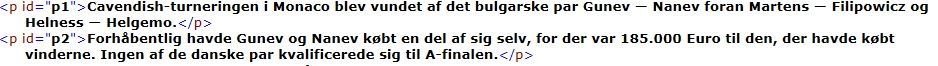
\includegraphics[scale=0.5]{figures/XmlIssue1}
 	\caption{Excerpt from the XML file containing the text found in appendix ~\ref{JPPOLHighestMatch1}.}
 	\label{XmlIssue1}
\end{figure}

\begin{figure}
	\centering
	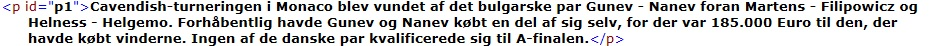
\includegraphics[scale=0.5]{figures/XmlIssue2}
	\caption{Excerpt from the XML file containing the text found in appendix ~\ref{JPPOLHighstMatch2}.}
	\label{XmlIssue2}
\end{figure}

Looking at figure ~\ref{JPPOLSencondHighestLCS} (the data from ~\ref{JPPOLSecondHighestScores}) we can see that again an almost perfect diagonal line is made, indicating that that these two articles are also close to identical. Once again we see the same pattern as before. The major part of the text is identical (see appendix ~\ref{JPPOLSencondHighestMatch1} and ~\ref{JPPOLSencondHighestMatch2} for article text), but we once again have some minor deviances. This once more being an white space issue, where the two XML files have been broken into paragraphs in different places. There is, however, a little interesting thing to note here. In the email address towards the end of the text part a white space have been inserted into one article, but not the other (figures ~\ref{XmlIssue3} and ~\ref{XmlIssue4}). This probably happened when the files were created, and is another error source that will appear from time to time. Like with the problem of white spaces and paragraphs, this will be unlikely to pose a serious source of errors, but should be kept in mind as well.

\begin{figure}
	\centering
	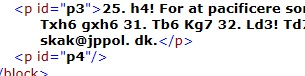
\includegraphics[scale=1.0]{figures/XmlIssue3}
	\caption{Excerpt of the XML file containing the data from article e410559d.}
	\label{XmlIssue3}
\end{figure}

\begin{figure}
	\centering
	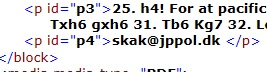
\includegraphics[scale=1.0]{figures/XmlIssue4}
	\caption{Excerpt of the XML file containing the data from article e410551d.}
	\label{XmlIssue4}
\end{figure}

Looking down the list of results there is a few interesting comparisons that have some scores, that makes it worth checking them out. The first of these we will look into is the comparison of articles \textit{e410557c} and \textit{e4105345}. This comparison scores relatively low with the Cosine algorithm, yet the LCS scores is pretty high (especially for the shortest article). The scores have been listed in table ~\ref{JPPOLPartialMatch}. We can also see the effect of having compared the length of the longest common substring with both the shortest and longest articles. No doubt that 38\% is a significant amount to have in common, but the 55\% really makes the score stand out. So what does this tell us? 

\begin{table}
\begin{center}
	\begin{tabular}{l | r}
	Ids & e410557c / e4105345\\ \hline
	Cosine & 0.407671899\\ \hline
	Basic LCS & 0.191534385\\ \hline
	LCS (long article) & 0.38342151\\ \hline
	LCS (short article) & 0.55743587\\ \hline
	Long article length & 2835\\ \hline
	Short article length & 1950\\ \hline	
	\end{tabular}
\end{center}
\caption{Scores for the 14th article comparison when comparing JP and POL sources (File: JPPOL.xlsx).}
\label{JPPOLPartialMatch}
\end{table}

First we will take a look on the LCS plot to try and get a visual indication of what could be going on. Figure ~\ref{ParticlaMatch} shows an excerpt of the LCS plot, the full plot is rather large, and would not fit in a single view in Excel. We will however not find any substrings with a length that fulfils the threshold outside the figure. The plot shows us that we have two articles that have quite a lot in common. Again we see issues with white spaces and also there are a few words words that breaks the longest common substrings. Overall we can say that the substrings found is sufficient identical and long (the breaks in between the substrings are quite short and the overall length of the substrings combined is rather long) to talk about a duplication. They only share an excerpt. That being said we also have a lot of text in the two articles that does not match, the match is therefore only partial. It is now obvious that we need to further divide the term \textit{'Match'} into subgroups, and we will do so later. When looking at the plot and then looking at the scores, we get a further explanation of what the scores tell us. The relative low Cosine score is influenced in part by the fact that there is quite a bit of text that is not shared by the articles, but also by the fact that the articles are of differing lengths.

\begin{figure}
	\centering
	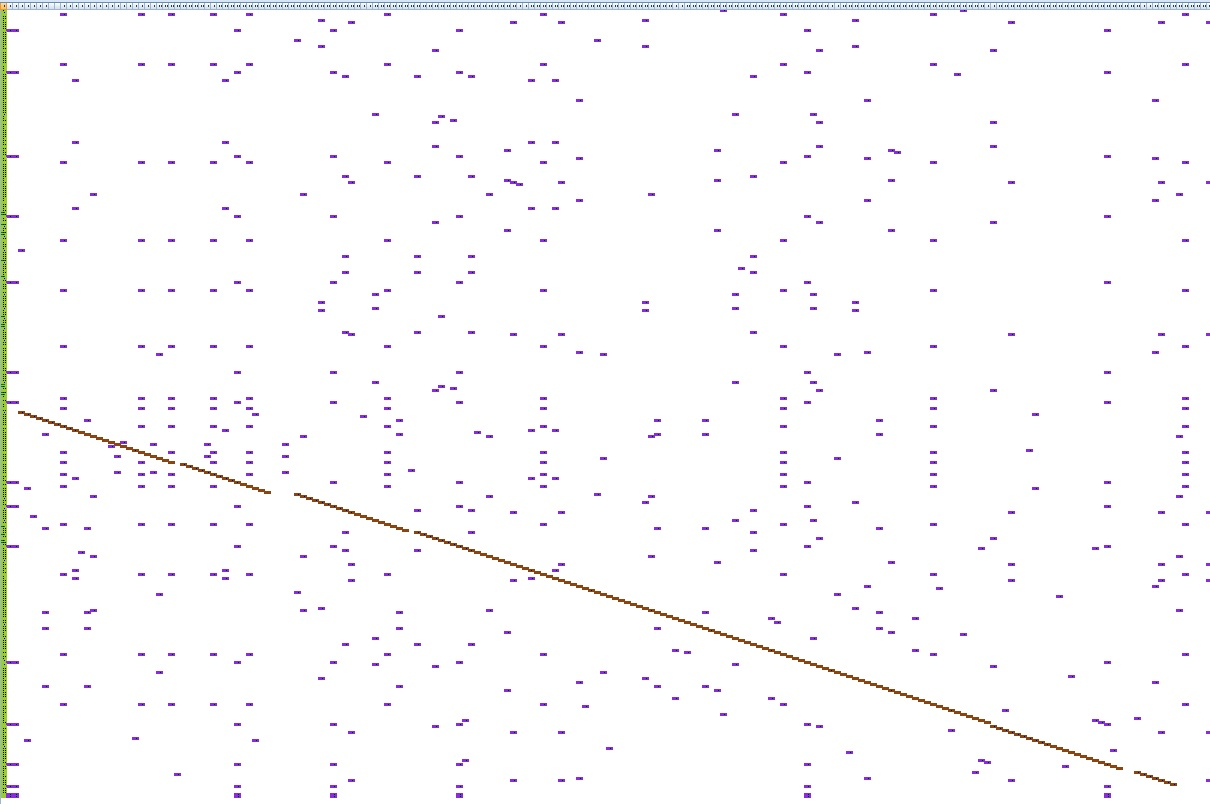
\includegraphics[scale=0.3]{figures/e410557c}
	\caption{LCS plot for the 14th article comparison in the set. The full plot is too big to be displayed in full in Excel, but the results can be seen in the file: e410557c-e4105345.xlsx.}
	\label{ParticlaMatch}
\end{figure}

The next comparison to be looked at is the 6th comparison (article Ids \textit{e410549c} and \textit{e4105515}). Here we have a fairly high Cosine score, but LCS scores are really low. The article lengths is fairly long, so we know it is articles that have some real content. The scores can be seen in table ~\ref{JPPOLSameContent}. Judging from the Cosine score, the articles have quite a bit in common, however the LCS score tells us that what ever they do have in common, is not expressed in sentences as such (we barely have any substrings in common). Once again we turn to the trusted to LCS plot to try and get an overview of what is going on.

\begin{table}
\begin{center}
	\begin{tabular}{l | r}
	Ids & e410549c / e4105515\\ \hline
	Cosine & 0.533468902\\ \hline
	Basic LCS & 0.0138186\\ \hline
	LCS (long article) & 0.013357899\\ \hline
	LCS (short article) & 0,017251637\\ \hline
	Long article length & 2171\\ \hline
	Short article length & 1681\\ \hline	
	\end{tabular}
\end{center}
\caption{Scores for the 6th article comparison when comparing JP and POL sources (File: JPPOL.xlsx).}
\label{JPPOLSameContent}
\end{table}

\begin{figure}
	\centering
	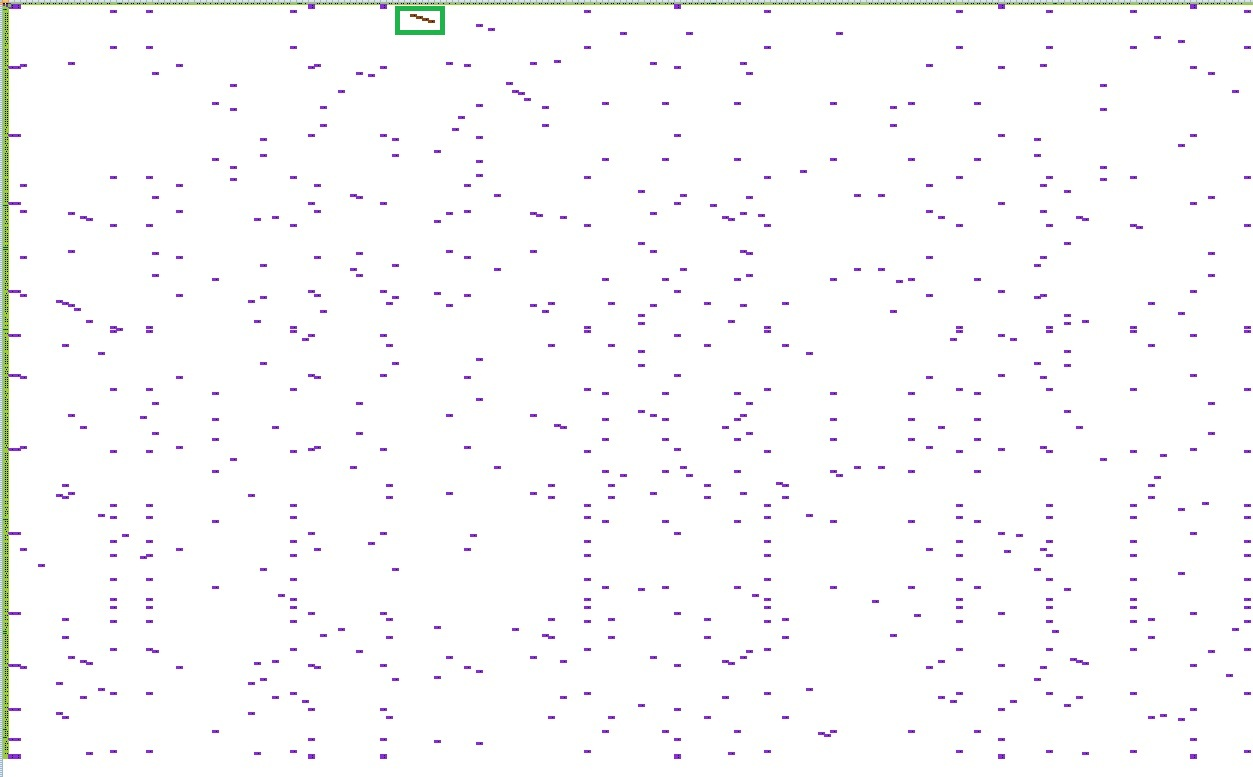
\includegraphics[scale=0.3]{figures/e410549c}
	\caption{LCS plot for the 6th article comparison in the set. The full plot is too big to be displayed in full in Excel, the full result can be seen in the file: e410549c-e4105515.xlsx. The only substring that is greater than the threshold have been marked in the green box.}
	\label{SameContent}
\end{figure}

In figure ~\ref{SameContent} we can see all substrings found, there is only one that is greater or equal to the threshold, it is marked in the green box. So the LCS plot does not tell us much about what is going on here, other than there truly is little in common in terms of substrings. We must then have a look at the article texts in order to see if we can figure out the reason for the relative high Cosine score. The two article's text can be found in appendix ~\ref{JPPOLSameContent1} and ~\ref{JPPOLSameContent2}. When reading the articles, it is clear that the articles is about the same topic (Brazilian footballer Carlos Bledorn Verri ('Dunga')), but are written in two different ways. If this started out with being a duplicate it has been obfuscated heavily, and it would be impossible to tell if that would be the reason. We can however say that the article have the same content, topic wise. A high (or relative high) Cosine score combined with a low LCS score, can then indicate that the article comparison are about the same topic, but without much other relation. This is something that we need to consider, and will get back to later.

\subsubsection{Low Scoring Comparison}
Finally for these sources an interesting case was found, when lowering the Cosine threshold to 0.1 (the results can be seen in the file: JYPPOL.xlsx). A comparison with the following scores was found ~\ref{JPPOLLowScoreMatch}. Both the Cosine and the LCS score for the longest article are really low. However looking at the LCS score for the short article a score of around 30\% is indicated. This would be a substantial part of the article that actually match the other article.

\begin{table}
\begin{center}
	\begin{tabular}{l | r}
	Ids & e41055d0 / e4105462\\ \hline
	Cosine & 0.105226949\\ \hline
	Basic LCS & 0,05952381\\ \hline
	LCS (long article) & 0,05952381\\ \hline
	LCS (short article) & 0,303030312\\ \hline
	Long article length & 168\\ \hline
	Short article length & 33\\ \hline	
	\end{tabular}
\end{center}
\caption{Scores for a low scoring (Cosine) comparison, with some interesting scores none the less. (File: JYPPOL.xlsx).}
\label{JPPOLLowScoreMatch}
\end{table}

When looking at the length of the articles, we can see that they are in fact quite short, the shortest being really short, only 33 characters long. This article will probably have very little interesting text (could be a breaking news article). Taking a look at the LCS plot helps to shed some light on the situation.

\begin{figure}
	\centering
	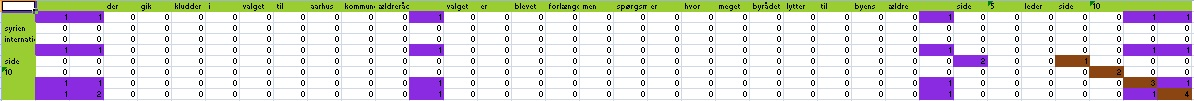
\includegraphics[scale=0.38]{figures/LengthIssue}
	\caption{LCS plot showing two very short articles being compared. This shows us an issue that can occur between the LCS score and the length of an article.}
	\label{LengthIssue}
\end{figure}

When looking at figure ~\ref{LengthIssue} we can see that the substring the two articles have in common are at the very end and is composed of the following: 
\begin{quote}
"side 10 \textvisiblespace \textvisiblespace"
\end{quote}

The short article (the word article used loosely here) does not contain any sort of informative text, other than a reference to the main article, and in such happened to have a very short substring in common with the other article. The substring just makes it to the threshold to be included, and one could consider from this to raise the threshold, but more testing into how inaccurate the results are from the current threshold is needed in order to see the overall impact of the threshold. But the length of the substring relative to the length of the article was enough to produce a substring that was just over 30\% of the article's length. So once again we must be aware of the length of the article, and this time also in combination with the LCS score. We must then ask the question is this a duplicate? To say it is not a match, is perhaps wrongful, but the contents of the short article would not really justify calling them a match. Later on we will try and look into how we can classify articles (in match groups) to giver a better indication of how well they match each other.

This example does show us, that interesting cases can be found in the comparisons that scores very low on the Cosine, but can still be a valid match (to some extend). In a future implementation, one should consider also looking into the low scoring comparisons.

\subsection{JV and FL Comparion}
In the following section, the article comparisons made from the sources JV and FL are being looked at. The file containing the results of this comparison is called JV-Lemvig.xlsx. A lot of the findings in this comparison will be similar to what was shown in the previous sections. We will therefore only look into results that brings something new to the table.

As there are many, many more comparisons in this set, the graph displaying the scores is incredible dense, and as it would be needed to scale it down, in order to make it fit the rapport, it would become nothing but a blur, so it will be left out of the chapter, the figure is instead found in appendix ~\ref{D3}.

The overall image of figure ~\ref{D3} is somewhat different from what we saw when comparing JP an POL. We are now seeing a lot of comparisons that looks to be matches, scoring high with both the Cosine and LCS algorithms. Now we are even seeing LCS scores that are greater than 1.0.

To look into why that is a closer inspection of the comparison seen in table ~\ref{JVFL100} is made.

\begin{table}
\begin{center}
	\begin{tabular}{l | r}
	Ids & e410c8b3 / e410c8c2\\ \hline
	Cosine & 0.929463029\\ \hline
	Basic LCS & 0.62894249\\ \hline
	LCS (long article) & 0.99072355\\ \hline
	LCS (short article) & 1,575221181\\ \hline
	Long article length & 539\\ \hline
	Short article length & 339\\ \hline	
	\end{tabular}
\end{center}
\caption{Scores for a low scoring (Cosine) comparison, with some interesting scores none the less. (File: JYPPOL.xlsx).}
\label{JVFL100}
\end{table}

The very high Cosine score indicates that a match has been found. Looking at the LCS scores, in particular the score for the shortest article, it is clear that the two article have a lot in common as the score indicates that the article shares 158\% of it's length with the other article. The articles are relative short, but not as short as to consider them having no "valuable" content. Again we turn to the trusted LCS plot to get a visual representation of the score.

\begin{figure}
	\centering
	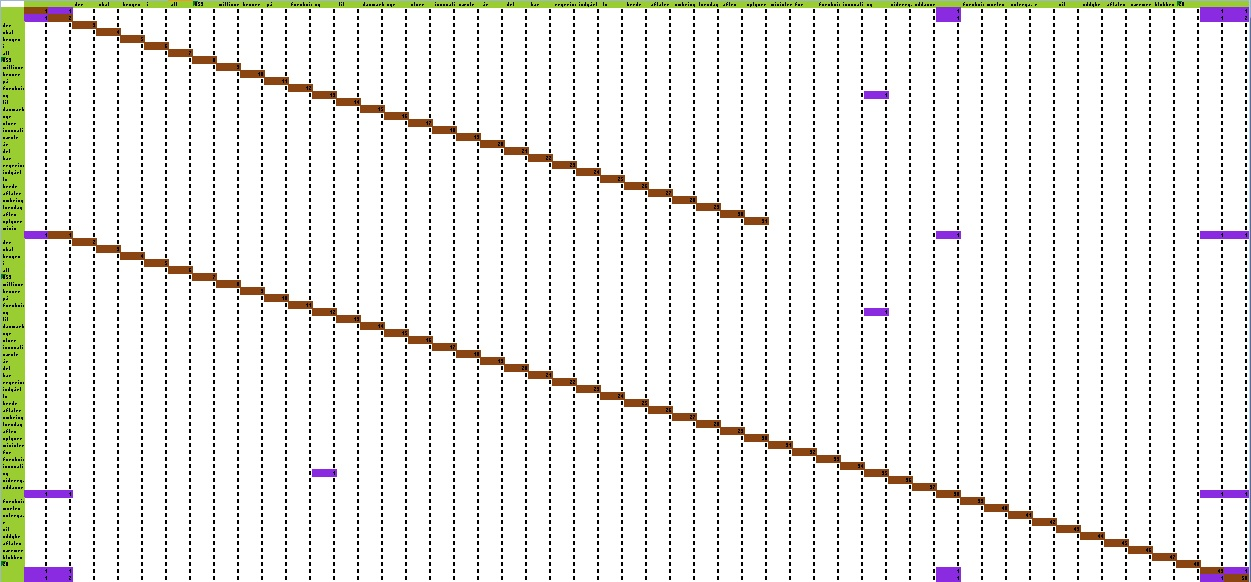
\includegraphics[scale=0.35]{figures/Over}
	\caption{LCS plotting showing what happens when text is repeated in the articles, we get an LCS score over 1.0.}
	\label{Over100}
\end{figure}

The plot in figure ~\ref{Over100} shows that we have two substrings of substantial length. When the substrings are placed in ways that they overlap in either direction, it means that text is repeated. This will often be the case when having a sub headline that are in turn repeated in the body text of the article (although it can also be a random collection of words, which all the purple squares shows). The text of the two articles can be found in appendix ~\ref{JVFLMatch1} and ~\ref{JVFLMatch2}. As it can be read from ~\ref{JVFLMatch2}, it has a lot of text repeated for some reason. This is the reason that the article scores more than 1.0 in the Cosine score. This result is not wrong per say, it just indicates that we have a lot of text in common in the articles being compared.

\section{Weighing the Scores}
In the previous sections we became aware that we need to do some amount of evaluation of various factors when determining if two articles are duplications. We need to take into account the length in combination with the scores, but also the scores in relation to each other. These factors all help us decide if we are looking at duplicates or not. In this section we will look into these factors and apply them to our comparisons.

In combination the two sets of scores (Cosine and both of the LCS scores) can draw us a more detailed picture, one that to a higher degree of confidence call tell about any relations between two articles. To try and break scores into something that is able to be defined, the following enums have been created, and called \textit{'Match Groups'}:

\begin{itemize}
\item \textbf{Match:} The comparison is to a high degree a perfect match, meaning that the two articles being compared have a lot of text in common, scores high with the algorithms and is somewhat similar in length.
\item \textbf{Partial Match:} This label would be a applied to a comparison, where only parts of the articles are shared, or that one article is a good deal shorter than the other, but scores highly in LCS. It would be considered an article excerpt.
\item \textbf{Same Content:} For comparisons with relative high Cosine scores, but somewhat low LCS scores, we can sometimes talk about the articles deal with the same topic, but without sharing much text. 
\item \textbf{Low Score Match:} Applying this label to a comparison would indicate that either one or both article are very short in length, can have a relative high Cosine score, but will have a high LCS score. It will indicate that the comparison most have a lot in common, but will maybe not contain much article text of much value.
\item \textbf{No Match:} When both algorithms scores low for a comparison, there is grounds to dismiss the comparison as a match. The articles will not have many sentences or special words in common.
\end{itemize}

The need for these match groups became obvious in the previous sections when we started to see comparisons that had a fairly high amount of text in common, but not enough to fully qualify as a duplicate.

The following table was created in order to try and give some weight to the scores. This could then be used in the program for score evaluation. The weight would be a factor that could be multiplied to the scores the algorithms produced in order to emphasize the result. These score weightings is based of tests that was done during the project.

\begin{table}
\begin{center}
	\begin{tabular}{l | c | c | c | c | c | c | c | c | c | c | r}
		    & 0.0 & 0.1 & 0.2 & 0.3 & 0.4 & 0.5 & 0.6 & 0.7 & 0.8 & 0.9 & 1.0\\ \hline
		0.0 & 0.01 & 0.01 & 0.01 & 0.01 & 0.01 & 0.01 & 0.01 & 0.01 & 0.01 & 0.01 & 0.01\\ \hline
		0.1 & 0.01 & 0.01 & 0.01 & 0.01 & 0.01 & 0.01 & 0.05 & 0.2 & 0.4 & 0.6 & 0.8\\ \hline
		0.2 & 0.01 & 0.01 & 0.05 & 0.1 & 0.1 & 0.1 & 0.3 & 0.5 & 0.6 & 0.8 & 0.85\\ \hline
		0.3 & 0.01 & 0.05 & 0.1 & 0.1 & 0.1 & 0.2 & 0.4 & 0.55 & 0.7 & 0.85 & 0.9\\ \hline
		0.4 & 0.01 & 0.05 & 0.1 & 0.1 & 0.1 & 0.2 & 0.4 & 0.6 & 0.75 & 0.85 & 0.95\\ \hline
		0.5 & 0.01 & 0.05 & 0.1 & 0.2 & 0.3 & 0.4 & 0.5 & 0.65 & 0.8 & 0.9 & 1.0\\ \hline
		0.6 & 0.01 & 0.07 & 0.1 & 0.2 & 0.4 & 0.5 & 0.6 & 0.7 & 0.85 & 0.9 & 1.0\\ \hline
		0.7 & 0.01 & 0.1 & 0.2 & 0.4 & 0.4 & 0.5 & 0.7 & 0.8 & 0.9 & 1.0 & 1.0\\ \hline
		0.8 & 0.01 & 0.1 & 0.4 & 0.6 & 0.7 & 0.8 & 0.8 & 0.9 & 1.0 & 1.0 & 1.0\\ \hline
		0.9 & 0.01 & 0.1 & 0.7 & 0.7 & 0.8 & 0.8 & 0.9 & 1.0 & 1.0 & 1.0 & 1.0\\ \hline
		1.0 & 0.05 & 0.2 & 0.8 & 0.8 & 0.9 & 0.9 & 1.0 & 1.0 & 1.0 & 1.0 & 1.0\\ \hline
	\end{tabular}
\end{center}
\caption{Score weights. The cosine score is the top most row and LCS score is the leftmost x axis. The weights indicates to what extend that articles have something in common. A low score would mean that the combination of Cosine and LCS score indicates that there is a low chance of any relation between the articles, a high score would mean the opposite. (File: Score Weight.xlsx)} \label{ScoreWeights}
\end{table}

The table ~\ref{ScoreWeights} would be an immediate indication as to how related two articles are, but we do also need to take another parameter into account, this being the length of the articles. A perfect match comparison would occur when two articles of the same length (roughly) and scoring close to 1.0 in both algorithms, but if two articles have a big difference in length that could affect the algorithm scores in a way that might not apply the right label when placing a comparison in a match group (as seen in figure ~\ref{LengthIssue}). The following enums was created to try and categorize articles by their length (table ~\ref{enums}).

\begin{table}
\begin{center}
	\begin{tabular}{l | c}
	Very Short & x < 300\\ \hline
	Short & x $\geq$ 300 $\bigwedge$ x < 500\\ \hline
	Medium & x $\geq$ 500 $\bigwedge$ x < 800\\ \hline
	Long & x $\geq$ 800 $\bigwedge$ x < 1200\\ \hline
	Very Long & x $\geq$ 1200\\ \hline
	\end{tabular}
\end{center}
\caption{Enums describing article length. X is the length of the article in characters and the values it is being compared with is the article length threshold for the various enums.}
	\label{enums}
\end{table}

\subsection{Applying the Score Weight}
Applying the weighing to the scores would only make sense if applied to the LCS score. The Cosine score is hard to alter in any meaningful way as it relates solely to the overall content matching. The LCS score can however become more useful if adjusted in accordance with the parameters discussed earlier. In the implementation only the LCS score based off the shortest article would be adjusted. This is because that this score would fluctuate more than the longer relative to it's length.

First off the article would be scored as normal. Once the post processing of the results would commence, all articles would get the enum describing their length. Then based of their length enums several methods was created to evaluate the LCS score based of the length and all of the comparisons scores. These methods was modelled in relation to table ~\ref{ScoreWeights}. The way it was modelled was to try and generate a lot of "buttons" that could be turned for many different cases of scores.

\lstset{style=sharpc}
\begin{lstlisting}[caption=Part of the method for applying LCS score weight, captionpos=b]
 class CalculateArticleScoreWeight
    {
        public float VeryShortVeryShort(float maxScore,
         float minScore, float shortArticleLength,
          float longArticleLength)
        {
            float factor = maxScore/minScore;
            if (shortArticleLength < 100 &&
             longArticleLength < 100)
            {
                if (factor > 0.8F && minScore > 0.7F)
                    return 1.0F;
                if (factor > 0.8F && minScore < 0.7F)
                    return 0.5F;
                return 0.1F;
            }

            if (shortArticleLength < 100 &&
             longArticleLength > 100)
            {
                if (factor > 0.8F && minScore > 0.6F)
                    return 1.0F;
                return 0.5F;
            }

            if (shortArticleLength > 100)
            {
                if (factor > 0.7F && minScore > 0.6F)
                    return 1.0F;
                return 0.6F;
            }
          }

\end{lstlisting}

<BESKRIV HVORDAN MATCHING GROUP BLEV TILSKREVET- KODE UDDRAG!!>



